%% The first command in your LaTeX source must be the \documentclass command.
\documentclass[acmtog]{acmart}
\usepackage[english,ngerman]{babel}
\usepackage[utf8]{inputenc}
\usepackage{plantuml}
\usepackage{listings}

%% \BibTeX command to typeset BibTeX logo in the docs
\AtBeginDocument{%
  \providecommand\BibTeX{{%
    \normalfont B\kern-0.5em{\scshape i\kern-0.25em b}\kern-0.8em\TeX}}}

\copyrightyear{2024}
\acmYear{2024}
\citestyle{acmauthoryear}

\usepackage[figurename=Fig.]{caption}
\setcopyright{none}
\makeatletter
\renewcommand{\fnum@figure}{Abb. \thefigure}
\makeatother
\addto\captionsngerman{\renewcommand{\figurename}{Abb.}}
\settopmatter{printacmref=false} % Removes citation information below abstract
\renewcommand\footnotetextcopyrightpermission[1]{} % removes footnote with conference information in first column

%%
%% end of the preamble, start of the body of the document source.
\begin{document}
\lstset{language=Java}

%%
%% The "title" command has an optional parameter,
%% allowing the author to define a "short title" to be used in page headers.
\title{Refactoring und technische Schulden in agilen Projekten}

%%
%% The "author" command and its associated commands are used to define
%% the authors and their affiliations.
%% Of note is the shared affiliation of the first two authors, and the
%% "authornote" and "authornotemark" commands
%% used to denote shared contribution to the research.
\author{Oliver Lindemann}
\authornote{Alle Studierenden trugen zu gleichen Teilen zu dieser Arbeit bei.}
\author{Tim Dietrich}
\authornotemark[1]
\author{Felix Herrling}
\authornotemark[1]
\affiliation{%
  \institution{Hochschule für Technik, Wirtschaft und Kultur Leipzig (HTWK Leipzig)}
  \streetaddress{Karl-Liebknecht-Str. 132}
  \city{Leipzig}
  %\state{Sachsen}
  \country{Deutschland}
  \postcode{04277}
}
%%
%% By default, the full list of authors will be used in the page
%% headers. Often, this list is too long, and will overlap
%% other information printed in the page headers. This command allows
%% the author to define a more concise list
%% of authors' names for this purpose.
\renewcommand{\shortauthors}{Lindemann, Dietrich und Herrling}

%%
%% The abstract is a short summary of the work to be presented in the
%% article.
\begin{abstract}

  Die vorliegende Arbeit untersucht das Konzept der technischen Schulden, deren
  Management in agilen Softwareentwicklungsprojekten und deren Rückzahlung durch
  Refactoring. Ausgehend von Ward Cunninghams Definition werden verschiedene Arten
  technischer Schulden kategorisiert und deren spezifische Eigenschaften wie Sichtbarkeit,
  Wert und Verzinsung analysiert. Die verschiedenen Möglichkeiten der Entstehung
  technischer Schulden werden mit Hilfe des “Technical Debt Quadrants” von Martin
  Fowler erörtert. Ein Schwerpunkt liegt auf dem technischen Schuldenmanagement (TSM)
  mit seinen Kernaktivitäten wie Identifizierung, Messung, Priorisierung und Rückzahlung.
  Hinzu kommen die Dokumentation und Kommunikation, bei denen deutlich wird, dass
  ein effektives Management technischer Schulden sowohl technische als auch
  organisatorische Maßnahmen erfordert. Aufbauend auf den Erkenntnissen zum Management
  technischer Schulden wird Refactoring als zentrale Methode zur Verbesserung der
  Codequalität und zum Abbau bzw. zur Prävention technischer Schulden untersucht.
  Die Arbeit betrachtet dabei sowohl theoretische Grundlagen und Best Practices des
  Refactorings als auch deren praktische Anwendung und Integration in agile
  Entwicklungsprozesse, um eine nachhaltige Softwareentwicklung zu gewährleisten.

\end{abstract}

\maketitle

\section{Einleitung und Motivation}

Diese Belegarbeit wurde im Rahmen des Masterstudiums Informatik an der HTWK Leipzig
im Modul Softwareengineering erstellt und befasst sich mit dem Thema: Refactoring und
technische Schulden in agilen Projekten. Dabei soll das Konzept der technischen Schulden
vertieft und deren Management in agilen Softwareentwicklungsumgebungen untersucht werden.
Aufbauend darauf sollen die Herausforderungen und Best Practices für regelmäßiges
Refactoring im Rahmen von Entwicklungsprozessen diskutiert werden.

Diese Arbeit ist folgendermaßen strukturiert.
In Kapitel \ref{sec:TS} wird das Konzept der technischen Schulden tiefgreifend untersucht.
Beginnend mit einer Einführung in Kapitel \ref{sec:EinführungTS} wird in Kapitel \ref{sec:BegriffTS}
der Begriff der technischen Schulden untersucht. Dabei wird auf die Aspekte Begriffsursprung, Gefahren, Entstehung, Kategorisierung und Eigenschaften eingegangen.
Anschließend wird in Kapitel \ref{sec:TSM} auf das Management von technischen Schulden eingegangen.
Dabei wird der Fokus auf die einzelnen Schritte des Technischen Schuldenmanagements gelegt.
Im folgendem Kapitel \ref{sec:Refactoring} wird dann eine Möglichkeit des technischen Schuldenmanagements in Form des Refactoring näher betrachtet.
Neben der Begriffsklärung wird hier die genaue Methodik beleuchtet, gefolgt von einer Betrachtung der Herausforderungen.
Danach werden die Erfolgsfaktoren näher betrachtet und eingeordnet.
Zuletzt folgt eine Zusammenfassung und Diskussion in Kapitel \ref{sec:Zusammenfassung}, sowie ein weiterer Ausblick in Kapitel \ref{sec:Ausblick}.

\section{Technische Schulden}\label{sec:TS}

\subsection{Einführung}\label{sec:EinführungTS}

Der Begriff “Technische Schulden” (TS) hat in Bezug auf (agile)
Softwareprojekte in den letzten Jahren und Jahrzehnten immer mehr an
Bedeutung gewonnen. Dies ist unter anderem darin begründet, dass das
Problem, welches technische Schulden darstellen, immer weiter anwächst.
Im Jahre 2010 wurden die globalen technischen Schulden auf 500 Milliarden
US-Dollar geschätzt\cite{Tom13}. Die Tendenz ist stark steigend. Im Folgenden soll
zunächst eine Begriffsdefinition und anschließend verschiedene Aspekte zu
technischen Schulden im Zusammenhang zu Softwareprojekten erörtert werden.

\subsection{Begriffsklärung}\label{sec:BegriffTS}

Eine eindeutige Definition von technischen Schulden stellt sich bei genauer
Betrachtung als sehr schwierig heraus. Je nach Quelle gibt es
unterschiedliche Aussagen dazu, was als technische Schuld zu sehen ist und
was explizit davon zu differenzieren ist \cite{Tom13}; \cite{Jaspan23}; \cite{Li14}. Außerdem hat sich im Laufe der
Zeit die Auffassung dieses Begriffs geändert. Allgemein kann man technische
Schulden als Rückstände in der Software während der Entwicklung bezeichnen,
welche die zukünftige Produktivität beeinflussen, also der Unterschied
zwischen dem aktuellen Zustand und einem ideal möglichen Zustand \cite{Brown10}.
Der Begriff TS ist dabei eine Metapher zu Schulden in der Finanzwelt und
soll den Grund für die steigenden Kosten in der Softwareentwicklung,
verständlich vor allem für Mitarbeiter aus nicht-technischen Berufsfeldern,
beschreiben \cite{Tom13}; \cite{Ylihuumo16}.

\subsection{Ursprung}\label{sec:UrsprungTS}

Die Metapher der technischen Schulden wurde erstmals in einem
Erfahrungsbericht von Ward Cunningham im Jahre 1992 verwendet \cite{Cunningham92}. Dieser
Bericht entstand im Rahmen eines Softwareprojekts der Firma Wyatt Software,
wobei das Programm “WyCASH+” für die Verwaltung von Portfolios in
Finanzmärkten entwickelt wurde. Cunningham schreibt:

\textit{“Shipping first time code is like going into debt. A little debt speeds
  development so long as it is paid back promptly with a rewrite.”} \cite{Cunningham92}

Dadurch wird das Prinzip ersichtlich. In Cunninghams Beispiel entstehen
technische Schulden dadurch, dass Software an den Endnutzer ausgeliefert
wird, obwohl diese noch nicht vollständig ausgereift ist. Dies ist dem
Entwicklerteam bekannt, wird jedoch willentlich in Kauf genommen. Dadurch
entstehen technische Schulden, welche später beglichen werden müssen. Der
Vorteil ist, dass dadurch schneller Feedback vom Kunden eingeholt werden
kann. Dadurch kann das Entwicklerteam neue Erfahrungen erhalten und
zukünftig bessere Entscheidungen treffen. Außerdem wird der
Entwicklungsprozess beschleunigt und die Qualität erhöht. \cite{Ylihuumo16}

\subsection{Gefahren technischer Schulden}\label{sec:GefahrenTS}

Der Begriff “Technische Schulden” war ursprünglich als Kommunikationsmittel
zwischen Software Entwicklern und Projektleitern gedacht. Für Projektleiter
sind interne Qualitätsaspekte der Software oft nicht gut verständlich bzw.
sichtbar. Zeitaufwände für Refactoring bringen keinen offensichtlichen Umsatz
oder neue Funktionalitäten und werden aus diesem Grund oft vermieden. \cite{Tom13}; \cite{Brown10}
Dies birgt Gefahren, da auf technische Schulden Zinsen, nämlich in Form von
Mehrkosten in der Zukunft, anfallen.

Cunningham schreibt hierzu: \textit{“The danger occurs when the debt is not repaid.
  Every minute spent on not-quite-right code counts as interest on that debt.”} \cite{Cunningham92}

Technische Schulden verursachen Mehraufwand im fortlaufenden Softwareprojekt,
wenn sie nicht rechtzeitig beglichen werden. Die Komplexität des Quellcodes
steigt, obwohl dies nicht notwendig ist. Dadurch entstehen Kosten und die
Produktivität sinkt. Die Entwicklung neuer Funktionen dauert länger und ist
fehleranfälliger. Außerdem wird die Qualität negativ beeinflusst. Im
Extremfall können diese Auswirkungen bis fast zum Erliegen des
Projektfortschrittes bzw. zum Scheitern führen. \cite{Tom13}; \cite{Ylihuumo16}

\subsection{Entstehung technischer Schulden}\label{sec:EntstehungTS}

Die Verwendung der Metapher der technischen Schulden hat sich im Laufe der
Zeit verändert. Ursprünglich noch als gezielte Maßnahme mit abwägbaren
Konsequenzen gedacht \cite{Tom13}, wird der Begriff heute weitreichender aufgefasst.
So gibt es beispielsweise unterschiedliche Meinungen dazu, ob schlechter Code
an sich als technische Schuld bezeichnet werden sollte, oder nicht. Martin
Fowler \cite{Fowler09} hat dazu folgendes Diagramm entworfen. Seiner Auffassung nach ist
es nicht sinnbringend, sich lange daran  aufzuhalten, ob ein aktuell
vorliegender Zustand eine technische Schuld darstellt oder nicht. Vielmehr
sollte man sich daran orientieren, ob die Verwendung der Metapher dabei helfen
kann, die Situation zu kommunizieren oder zu verbessern. Diese Auffassung wird
auch im weiteren Verlauf dieser Ausarbeitung verfolgt. Durch das Diagramm
werden die Gründe für die Entstehung technischer Schulden in 4 allgemeine
Kategorien (Quadranten) eingeteilt.

\begin{figure}[t]
  \centering
  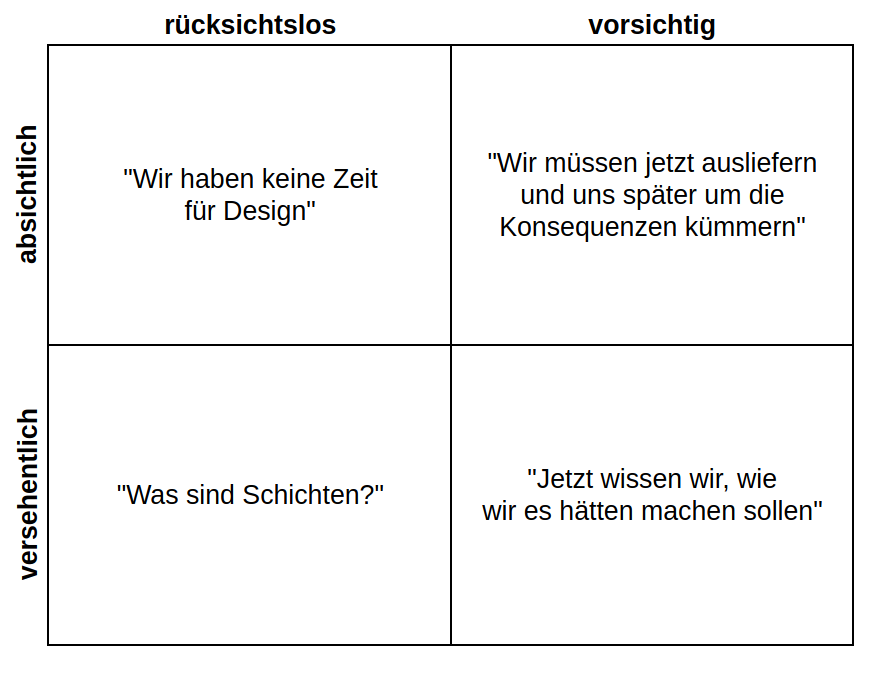
\includegraphics[width=\linewidth]{images/Uebersetzung_TS_Quadrant.png}
  \caption{Technical Debt Quadrant nach \cite{Fowler09}}
  \label{fig:Quadrant_TS}
  \Description{Technical Debt Quadrant nach \cite{Fowler09}}
\end{figure}

Absichtliche, rücksichtslose TS werden meistens nicht abgewägt. Dies bedeutet
jedoch nicht zwingend, dass die technischen Schulden unbewusst aufgenommen
werden. Oftmals sind bessere Methoden und Praktiken bekannt, werden jedoch
nicht angewandt. Ein Beispiel hierfür sind allgemeine “Quick and dirty”-Lösungen.
Gründe können feste Ausliefertermine oder Meilensteine im Projekt sein, die
unbedingt eingehalten werden müssen.

Versehentliche, rücksichtslose TS entstehen vor allem durch Unwissenheit und
fehlende Kompetenz im Entwicklerteam. Dies ist besonders gefährlich, da die
Schulden unbewusst aufgenommen werden und deshalb wahrscheinlich nicht in
einem vernünftigen zeitlichen Rahmen abgebaut werden.

Absichtliche, vorsichtige TS bezeichnet im Allgemeinen die technische Schuld
nach dem Vorbild Cunninghams. Die technische Schuld wird bewusst aufgenommen.
Vor- und Nachteile werden dabei abgewägt. Im Optimalfall wird auch direkt ein
Plan zum Abbau der Schuld aufgestellt. Diese Schuld entsteht z.B. wenn feste
Ausliefertermine eingehalten werden müssen oder anderweitige
Ressourcenknappheit besteht.

Versehentliche, vorsichtige TS entsteht in jedem Projekt. Ein Projekt ist
immer auch ein Lernprozess für alle beteiligten Mitarbeiter. Dabei werden
neue Erkenntnisse gewonnen, durch welche der Quellcode optimiert werden kann.
So entsteht technische Schuld, welche erst nach Abschluss des Projektes
erkannt wird. Dies kann nicht vermieden werden, egal wie sorgfältig geplant
und gearbeitet wird.

\subsection{Kategorisierung technischer Schulden}\label{sec:KategorisierungTS}

Technische Schulden können in verschiedenen Arten auftreten. Ein einheitliches,
anerkanntes  Modell zur Kategorisierung gibt es nicht. Je nach Studie, Methodik
und Umfeld unterscheiden sich die Ergebnisse zur Kategorisierung. Die
folgende Auflistung ist das Ergebnis sowohl aus praktischen Analysen \cite{Jaspan23} als
auch aus wissenschaftlicher Arbeit \cite{Li14}. Dabei wurde eine Auswahl der
wichtigsten Kategorien getroffen, sodass die hier gegebene Übersicht nicht
vollständig ist. Weiterhin ist es möglich, die einzelnen Kategorien noch
feiner aufzuspalten. Dies würde an dieser Stelle zu weit führen und wird
deshalb nicht gemacht. Für weitere Informationen wird auf die genannten
Quellen verwiesen.

Die am häufigsten vorkommende Art technischer Schuld besteht im Zusammenhang
mit dem \textbf{Quellcode}. Hierzu zählen unter anderem schlechter Code, Duplikate,
zu hohe Komplexität, nicht verwendeter Code und veralteter oder toter Code.
Die Ursachen hierfür sind vielfältig, beispielsweise mangelnde Kompetenz im
Entwicklerteam oder Zeitdruck.

Schulden in der \textbf{Architektur} wirken sich stark auf die Wartbarkeit und
Erweiterbarkeit des Projektes aus. Cunninghams ursprüngliche Definition fällt
in diese Kategorie. Er erklärt, wie die Architektur vorerst nur für neue
Features angepasst und später für das gesamte Projekt bereinigt wurde \cite{Cunningham92}.

\begin{figure}[t]
  \centering
  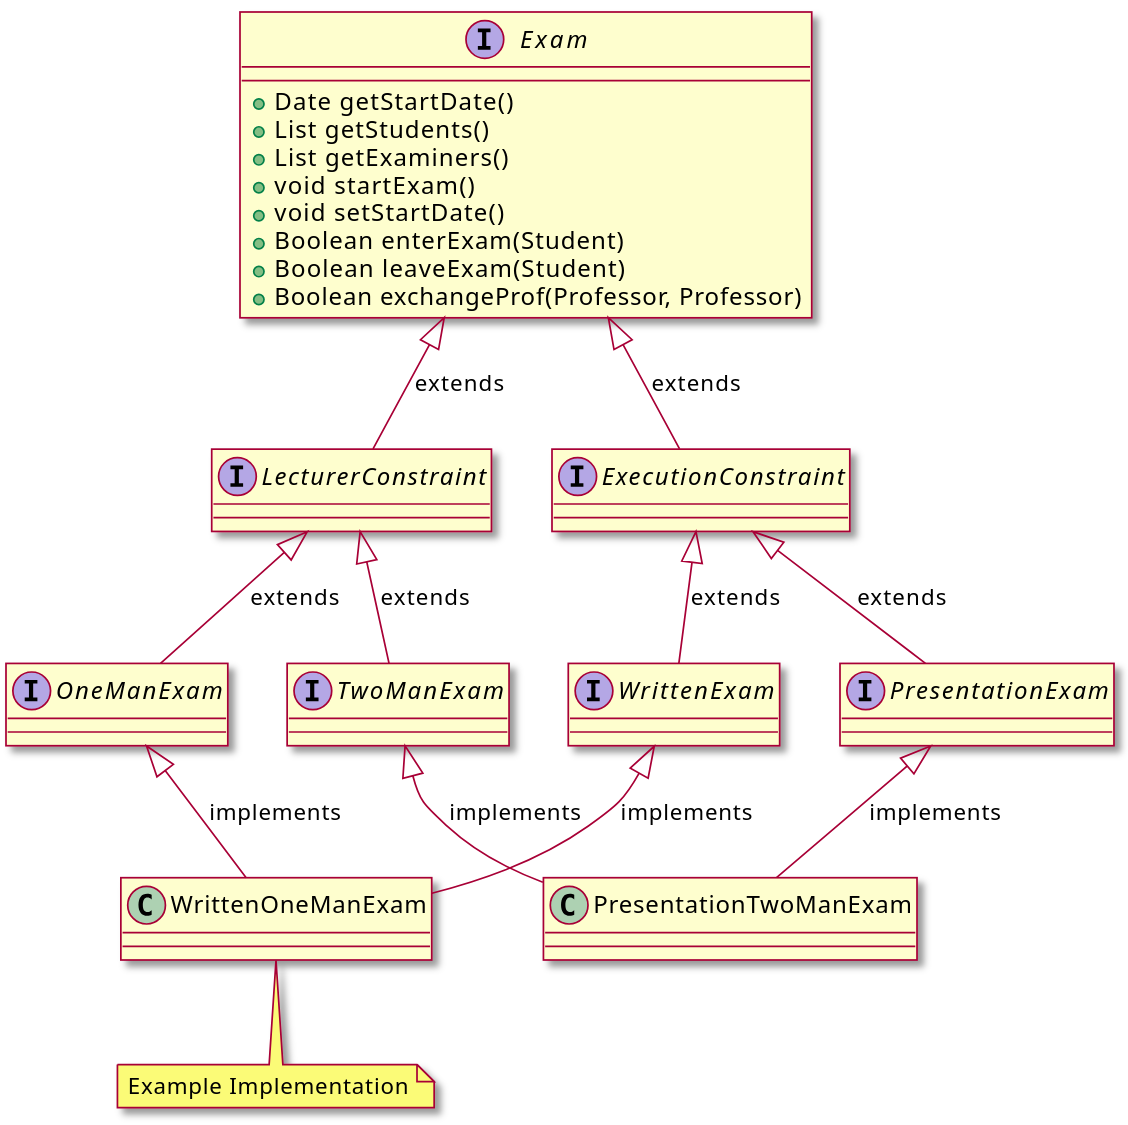
\includegraphics[width=\linewidth]{images/ArchitectureExample01.png}
  \caption{Beispiel TS in der Architektur}
  \label{fig:BeispielArchitektur_TS}
  \Description{Beispiel TS in der Architektur}
\end{figure}

Abbildung \ref{fig:BeispielArchitektur_TS} zeigt ein Klassendiagramm welches im
Modul Softwareengineering entstanden ist. Aufgabe war die Umsetzung einer Architektur
für verschiedene Prüfungsarten an einer Hochschule. Gefordert war dabei, dass die
Architektur einfach und schnell für neue Prüfungsarten erweitert werden kann. Dies
wird durch verschiedene Interfaces realisiert: eine neue Prüfung kann nach Bedarf
durch Implementierung der benötigten Interfaces umgesetzt werden. Die Lösung scheint
für die gestellten Forderungen passend zu sein. In einer neuen Anforderung soll es
nun ermöglicht werden, dass gewisse Attribute der Prüfung nach Prüfungsstart nicht
mehr geändert werden dürfen. Dies ist mit der aktuellen Struktur schlecht umzusetzen.
Hier wird eine technische Schuld sichtbar, welche erst durch die Anforderungsänderung
erkannt werden kann.

\begin{figure}[t]
  \centering
  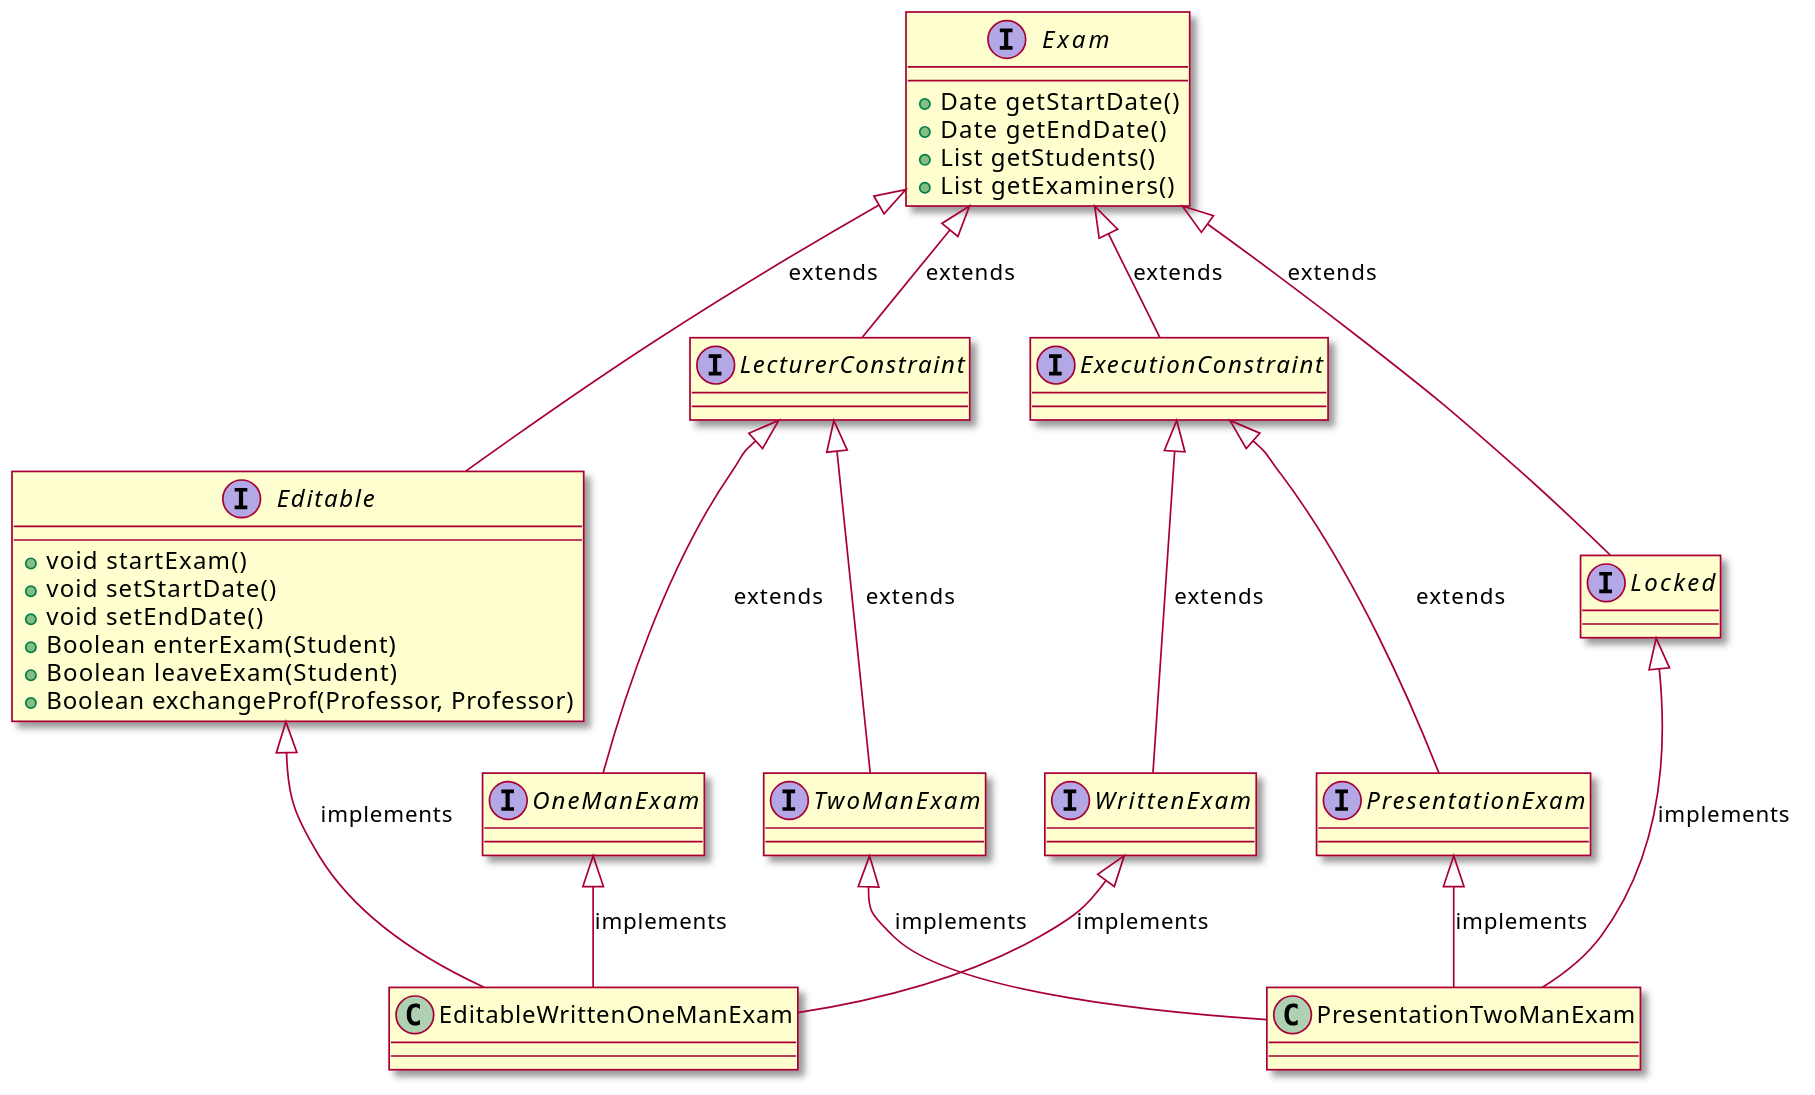
\includegraphics[width=\linewidth]{images/ArchitectureExample02.png}
  \caption{mögliche Lösung für die TS}
  \label{fig:BeispielArchitektur_TS02}
  \Description{mögliche Lösung für die TS}
\end{figure}

Abbildung \ref{fig:BeispielArchitektur_TS02} zeigt eine mögliche Lösung für diese 
technische Schuld. Die Architektur wird um zwei weitere Interfaces 'Editable' und 
'Locked' erweitert. Die Setter-Funktionen werden in das Editable-Interface verschoben. 
Die implementierenden Klassen können dann je nach Bedarf eines dieser Interfaces 
implementieren um die gewünschte Funktionalität zu erreichen.


Rückstände bei \textbf{Tests} beinhalten unter anderem Unit-Tests, Integrationstests
und Akzeptanztests. Tests werden aus zeitlichen Gründen oft vernachlässigt,
jedoch bleiben durch fehlende Tests potentiell mehr Bugs unerkannt, wodurch
sich unerkannte technische Schuld aufbauen kann. Der Abbau dieser Schuld ist
später kostenintensiver, als die zeitliche Ersparnis durch das Auslassen der
Tests.

Dies kann beispielsweise bei folgender Klasse passieren. die Klasse Timeslot
speichert eine Start- und eine Endezeit als Zeitslot ab. Zudem bietet sie
eine Möglichkeit zum Abfragen der Dauer des Zeitslots.

\begin{lstlisting}[frame=single,breaklines=true]
public class Timeslot {

  public LocalDateTime start;
  public LocalDateTime end;

  public Timeslot(LocalDateTime start,
                  LocalDateTime end) {
    this.start = start;
    this.end = end;
  }

  public Duration getDuration() {
    return Duration.between(start, end);
  }
}
\end{lstlisting}

Diese Klasse sieht zwar auf den ersten Blick sehr überschaubar aus,
enthält aber unerwartetes Verhalten bei Eingaben von null-Werten.
Dies kann mit einer einfachen Abfrage verhindert werden:

\begin{lstlisting}[frame=single,breaklines=true]
  public Timeslot(LocalDateTime start,
                  LocalDateTime end) {
    if (start == null || end == null) {
      throw new IllegalArgumentException();
    }

    this.start = start;
    this.end = end;
  }
\end{lstlisting}

Auch wenn null-Werte nun geprüft werden, kann es zu weiteren Problemen
kommen. So wird die Richtigkeit der gegebenen Datumsangaben nicht
geprüft, etwa dass der Endzeitpunkt nicht vor oder gleich dem
Startzeitpunkt ist.

\begin{lstlisting}[frame=single,breaklines=true]
  public Timeslot(LocalDateTime start,
                  LocalDateTime end) {
    if (start == null || end == null) {
      throw new IllegalArgumentException();
    }

    if (!end.isAfter(start)) {
      throw new IllegalArgumentException();
    }

    this.start = start;
    this.end = end;
  }
\end{lstlisting}

Mit umfangreichen Tests kann die Richtigkeit auch bei kleinen, übersichtlichen
Klassen sichergestellt werden. Anzumerken ist jedoch, dass durch die oben
getägtigten Veränderungen ebenso neue technische Schulden eingeführt werden können.
So wird bei der null-Prüfung nicht unterschieden, welcher der geprüften Werte null ist
und eine uneindeutige Fehlermeldung erzeugt. Dies führt zu einer neuen technischen
Schuld, beispielsweise bei einer etwaigen Darstellung des Fehlers.

Veraltete, unvollständige oder falsche \textbf{Dokumentation} ist ebenfalls eine
Kategorie der technischen Schulden. Hierzu zählen auch aussagekräftige
Kommentare im Quellcode. Die Bedeutung guter Dokumentation wird z.B. dann
ersichtlich, wenn neue Mitarbeiter zum Projekt hinzugefügt werden. Gute
Dokumentation beschleunigt den Einarbeitungsprozess und erhöht die
Produktivität. Schlechte Dokumentation erhöht die Gefahr für Fehler und
Missverständnisse und erschwert die Wartbarkeit. Ein Fallbeispiel dazu kann
in \cite{Brown10} gefunden werden. Dort wird ein Softwareprojekt beschrieben, das über
längere Zeit von einem einzelnen Entwickler durchgeführt wurde. Das
Unternehmen hatte allgemeine Vorschriften für Dokumentation, Architektur und
Quellcode. Die Ergebnisse des Projekts waren immer zufriedenstellend, d.h.
es gab wenige Defekte und einen stetigen Fortschritt bezüglich der
umgesetzten Anforderungen. Das Projekt wurde später von einem neuen
Entwicklerteam übernommen. Dabei wurde festgestellt, dass von den
unternehmensinternen Vorgaben stark abgewichen wurde. Das neue
Entwicklerteam muss diese technische Schuld nun begleichen, indem sie den
Quellcode verstehen und entsprechend der Vorgaben anpassen. Die Umsetzung
neuer Anforderungen wird dadurch verzögert.

Technische Schulden bezüglich der \textbf{Anforderungen} bezeichnet im Allgemeinen den
Unterschied zwischen dem aktuellen Fortschritt und den in der Spezifikation
definierten Features und Funktionen. Diese Schuld wird beispielsweise dann
ersichtlich, wenn die Entwicklung einzelner Features aufeinander aufbaut und
somit bei Verzögerung der zugrundeliegenden Features beeinflusst wird. Dies
beinhaltet sowohl fehlende, als auch unvollständig oder fehlerhaft umgesetzte
Anforderungen.

Unter die Kategorie \textbf{Infrastruktur} fallen Systeme, Konfigurationen,
Anwendungen und Werkzeuge, welche vom Entwicklerteam verwendet werden.
Schulden dieser Kategorie beeinflussen die Produktivität, z.B. durch komplexe
Build-Prozesse, schlechtes Management der Dependencies oder mangelhafte
Versionierung.

\subsection{Eigenschaften technischer Schulden}\label{sec:EigenschaftenTS}

Um einen guten Umgang mit technischen Schulden zu ermöglichen, ist es
notwendig, diese zu charakterisieren und Eigenschaften zu definieren. Hierzu
gibt es keine allgemeingültigen Modelle. Die Analyse von technischen Schulden
verwendet immer wieder Parallelen zu finanziellen Schulden. \cite{Brown10}; \cite{Li14}

Die \textbf{Sichtbarkeit} beschreibt, wie einfach und schnell eine technische Schuld
erkannt werden kann. Defizite wie Bugs oder fehlende Funktionen sind eventuell
einfacher zu erkennen, wohingegen Rückstände in der Dokumentation oder
Softwarearchitektur mitunter länger unerkannt bleiben. Besonders bei schlecht
sichtbaren technischen Schulden ist es wichtig, diese bereits bei der
Entstehung wahrzunehmen und die Behebung einzuplanen.

Der \textbf{Wert} der technischen Schuld beschreibt die Differenz zwischen dem
aktuellen Zustand und dem idealen Zustand. Aufbauend darauf kann der Zeitwert
beschrieben werden, welcher zusätzlich die angefallenen Zinsen, in Form von
Kosten und Zeit, beinhaltet. Dabei ist es schwer bis unmöglich, einen
konkreten Zahlenwert zu definieren.

Die \textbf{Verzinsung} beschreibt, wie stark der Wert der technischen Schuld ansteigt,
wenn diese nicht beglichen wird. Auch hier ist es schwer, einen genauen
Zahlenwert festzulegen. Vielmehr ist es sinnbringend, den allgemeinen Verlauf
der Steigerung zu betrachten, z.B. linear oder exponentiell. Dies kann dann
zur Priorisierung verwendet werden. Vor allem exponentiell ansteigende
technische Schulden besitzen ein Potential für Disaster, weil sie die
Produktivität auf ein Minimum reduzieren können.

Technische Schulden werden immer in einem bestimmten \textbf{Umfeld} aufgenommen.
Dies kann beispielsweise Software Architektur, Tests oder Dokumentation sein.

Die \textbf{Herkunft} der technischen Schuld wurde bereits in Abschnitt \ref{sec:EntstehungTS} erklärt
und soll hier deshalb nur nochmal erwähnt werden.

Der \textbf{Einfluss} bezieht sich darauf, wie viele Komponenten der Software
betroffen sind. Weitreichende technische Schulden steigen oftmals schneller
und stärker im Wert und benötigen mehr Ressourcen, um behoben zu werden.


\section{Technisches Schuldenmanagement}\label{sec:TSM}

Technisches Schuldenmanagement (TSM, engl. Technical Debt Management) beschreibt
einen Ansatz, um sowohl potenzielle technische Schulden präventiv zu vermeiden
als auch bestehende Schulden zu verwalten und zu reduzieren. TSM kann dabei in
die folgenden Aktivitäten unterteilt werden: Identifikation, Messung, Priorisierung,
Prävention, Überwachung, Dokumentation und Kommunikation sowie Rückzahlung. \cite{Alves16}

\subsection{Identifizierung}\label{sec:TSM_Identifizierung}
Der erste Schritt im TSM ist die Identifizierung von technischen Schulden
und bildet die Grundlage für deren weitere Verwaltung. Dies umfasst sowohl
die absichtlich als auch die unabsichtlich durch technische Entscheidungen
verursachten technischen Schulden. Manuelle Code-Reviews und automatische
Code-Analysen können dabei helfen, technische Schulden im Code zu erkennen.
Dies können bspw. Verstöße gegen Programmierrichtlinien oder fehlende Tests sein.
Um jedoch auch technische Schulden auf Architektur, Design- oder Anforderungsebene
zu erkennen, kann auf verschiedene Indikatoren geachtet werden. Beispiele hierfür
sind Verstöße gegen die Modularität, Gott-Klassen oder Abhängigkeiten von
Softwarekomponenten. \cite{Alves16}

\subsection{Messung}\label{sec:TSM_Messung}
Die Messung technischer Schulden zielt darauf ab, die Auswirkungen der
identifizierten Schulden zu quantifizieren. Dies kann durch die mathematische
Berechnung oder definierte Modelle geschehen, aber auch durch die Abschätzung
durch menschliche Erfahrung und Expertise. Betrachtet werden dabei insbesondere
der Wert ("principal") und die Zinsen ("interest") einer technischen Schuld,
die den Aufwand zur Tilgung (Rückzahlungskosten) sowie die potentiellen Kosten
durch Aufschiebung/Nicht-Rückzahlung oder erhöhte Komplexität beschreibt. \cite{Alves16}


\subsection{Priorisierung}\label{sec:TSM_Priorisierung}

Für die Entscheidungsfindung, welche TS zuerst beglichen bzw. aufgeschoben
werden sollten, werden diese priorisiert. Hierzu werden verschiedene theoretische
Ansätze und Modelle herangezogen. Besonders häufig zitiert und in der Literatur
diskutierte Modelle umfassen: \cite{Seaman12}

\textbf{Kosten-Nutzen-Analyse} (Cost-Benefit Analysis)
Die Kosten-Nutzen-Analyse basiert auf der Erstellung einer Liste aller technischen
Schulden.Für jede Schuld werden der Aufwand für die Behebung (Wert) und die
potenziellen Zusatzkosten bei Nichtbehebung (Zinsen) geschätzt. Auf Grundlage dieser
Daten wird eine Kosten-Nutzen-Matrix erstellt, mit der technische Schulden priorisiert
werden können. Dabei werden vor allem solche Schulden bevorzugt, deren Nutzen durch
die Behebung hoch ist, während die Behebungskosten vergleichsweise gering sind. \cite{Seaman12, Alves16}

\textbf{Portfolio-Ansatz}
Der Portfolio-Ansatz überträgt Prinzipien aus der Finanzwelt auf das Management
technischer Schulden. Ähnlich wie bei finanziellen Investitionen wird ein Portfolio
erstellt, das verschiedene technische Schulden mit ihren jeweiligen Risiken und
potenziellen Vorteilen abbildet. Ziel ist es, die Risiken gezielt zu streuen und
den Nutzen durch eine strategische Priorisierung zu maximieren. Grundlage des Ansatzes
ist eine detaillierte Liste der technischen Schulden, die folgende Informationen enthält:
\begin{itemize}
  \item die Position der Schuld (Modul, Datei)
  \item Zeitpunkt der Entdeckung
  \item Verantwortliche Person
  \item Betrag der TS (Kosten für die Behebung)
  \item Geschätzte Zinsen und deren Wahrscheinlichkeit
\end{itemize}
Basierend auf dieser Liste wird bei jedem Software-Inkrement entschieden,
welche Schulden zurückgezahlt und welche aufgeschoben werden. \cite{Seaman12, Alves16}

\textbf{Optionsstrategie}
Die Optionsstrategie betrachtet die Behebung technischer Schulden als
strategische Investition, bei der kurzfristige Kosten in Kauf genommen
werden, um langfristige Vorteile und Flexibilität zu erzielen. Dabei
wird jede technische Schuld als eine Art Option betrachtet, bei der es
möglich ist, die Rückzahlung aufzuschieben, bis Änderungen am betroffenen
Systemteil erforderlich sind. Diese Strategie eignet sich für technische
Schulden, deren zukünftige Relevanz oder Auswirkungen derzeit noch
unsicher sind. \cite{Seaman12, Alves16}

\textbf{Anaytic Hierarchy Process} (AHP)
Der Analytische Hierarchieprozess vergleicht technische Schulden anhand
vordefinierter, gewichteter Kriterien, wie Zinsen, Aufwand und Auswirkungen
auf die Softwarequalität. Durch Paarweise Vergleiche wird eine Rangfolge
erstellt, die die Priorität jeder Schuld abbildet. Ergebnis ist eine klare
Übersicht, welche Schulden zuerst zurückgezahlt werden sollten. \cite{Seaman12, Alves16}


Die Kosten-Nutzen-Analyse und der Portfolio-Ansatz werden in Studien am
häufigsten zitiert. Wie häufig diese theoretischen Modelle in der Praxis jedoch
zum Einsatz kommen, kann nicht gesagt werden, da hierzu die Studienlage
unzureichend ist. \cite{Seaman12} Teils wird nach eigenem Ermessen oder vom
jeweiligen Unternehmen selbst festgelegten Kriterien entschieden, welche TS
priorisiert und behandelt werden. So kann eine TS am wichtigsten kategorisiert
werden, wenn diese kundenbezogen sind oder andere (Entwicklungs-)arbeiten
behindern. \cite{Codabux13}

\subsection{Prävention}\label{sec:TSM_Prävention}
Um technische Schulden von vornherein zu vermeiden und die Qualität sowie
Wartbarkeit von Software sicherzustellen, können bei der Entwicklung
beispielsweise automatisierte Tests, Coding-Guidelines, Code-Reviews und
eine einheitliche Definition of Done (DoD) eingesetzt werden. Diese und
weitere Methoden der Qualitätssicherung sollen sicherstellen, dass bereits
während des Entwicklungsprozesses möglichst wenig technische Schulden
entstehen, wodurch langfristig auch der Aufwand für deren spätere Reduktion
minimiert wird. \cite{Behutiye17, Holvitie18, Alves16}

\subsection{Überwachung}\label{sec:TSM_Überwachung}
Die Überwachung und kontinuierliche Beobachtung identifizierter, aber noch
nicht beglichener technischer Schulden gehören zu den Kernaufgaben des TSM,
da ohne sie keine fundierten Entscheidungen für andere TSM-Aktivitäten getroffen
werden können \cite{Ernst15}. Dies setzt jedoch die vorhergehende Messung der
technischen Schulden voraus, da eine Überwachung ohne entsprechende Datengrundlage
und messbare Werte nicht möglich ist. \cite{Alves16} Zumeist wird beobachtet,
wie sich der Wert und die Zinsen einer technischen Schuld über die Zeit verändern
und ob technische Schulden aufgenommen oder abgebaut werden. Je nach Datenlage
kann entschieden werden, ob der Fokus stärker auf den Abbau technischer Schulden
gelegt wird oder nicht. Entscheidungshilfe kann zudem das Beobachten der
Gesamtqualität der Software und die Produktivität des Entwicklungsteams liefern.
Auch Tools können bspw. bei den technischen Aspekten wie Code-Dopplungen,
fehlende Kommentare, Verstöße gegen Programmierrichtlinien oder potenzielle
Bugs helfen. \cite{Ylihuumo16, Alves16}

In der Praxis wird die Überwachung selten konsequent umgesetzt. Hauptursache
ist die fehlende Messung technischer Schulden und die daraus resultierende
unzureichende Datengrundlage für eine Beobachtung. \cite{Ylihuumo16}

\subsection{Dokumentation}\label{sec:TSM_Dokumentation}
Die Dokumentation im TSM stellt sicher, dass alle relevanten Informationen über
technische Schulden transparent, nachvollziehbar und für alle Beteiligten
zugänglich sind. Dies kann beispielsweise über ein Tool wie JIRA oder ein
separates Backlog geschehen. So wird sichergestellt, dass bereits identifizierte
technische Schulden nicht in Vergessenheit geraten, sondern mit in den
Entwicklungsprozess eingeplant und zurückgezahlt werden können. Darüber hinaus
unterstützt die Dokumentation auch andere Schritte des TSM wie bspw. die
Überwachung, da sie einen zentralen und definierten Ort bereitstellt,
an dem alle identifizierten technischen Schulden zusammengetragen sind.
Zur Dokumentation zählt dabei häufig eine eindeutige ID, der Ort, Typ
und Beschreibung der Schuld, eine verantwortliche Person, der Wert und
die Zinsrate sowie das Datum.

\subsection{Kommunikation}\label{sec:TSM_Kommunikation}
Die alleinige Dokumentation technischer Schulden reicht jedoch häufig nicht
aus, um deren Risiken auf den weiteren Projektverlauf allen Stakeholdern
erkenntlich zu machen. Angefangen im Entwicklerteam ist es wichtig,
regelmäßig über die technischen Schulden des Projekts zu sprechen,
um sicherzustellen, dass alle Teammitglieder ein gemeinsames Verständnis
über die Prioritäten und den Status der Schulden haben. Behilflich können
dabei bspw. regelmäßige Reviews und Retrospektiven sein, bei denen technische
Schulden diskutiert und mögliche Ursachen erkannt und zukünftig vermieden werden können.
Damit technische Schulden nicht nur innerhalb des Teams dokumentiert, sondern auch
gegenüber der Geschäftsleitung und anderen Stakeholdern klar und transparent aufgezeigt
werden können, ist eine klare Kommunikation erforderlich. Diese muss die Wichtigkeit
der Einbeziehung von Rückzahlungen technischer Schulden in den Entwicklungsprozess
verdeutlichen. Die Vermittlung zwischen technischen und nicht-technischen Stakeholdern
stellt dabei eine große Herausforderung dar. Nicht-technischen Stakeholdern,
welche zumeist auf kurzfristige Ziele wie die Veröffentlichung neuer Features
konzentriert sind, müssen die Folgen technischer Schulden (z.B. Sicherheit gefährdet,
erhöhter Entwicklungsaufwand) vermittelt werden. Eine effektive Kommunikation hilft
dabei, die Wichtigkeit der regelmäßigen Rückzahlung technischer Schulden zu verdeutlichen
und die Entscheidungsträger in den Prozess einzubinden. \cite{Ylihuumo16, Alves16}

\subsection{Rückzahlung}\label{sec:TSM_Rückzahlung}
Als letzten Schritt im technischen Schuldenmanagement steht die Rückzahlung von
technischen Schulden. Diese erfolgt je nach Typ der technischen Schuld. So kann
einfaches Bug-Fixing bei fehlerhaftem Code zum Einsatz kommen, wohingegen bei
tieferliegenden Problemen, neuen oder geänderten Anforderungen Reengineering,
Rewriting oder Refactoring zum Einsatz kommen kann. In der Praxis wird dabei
am häufigsten auf Refactoring zurückgegriffen, um technische Schulden zu
begleichen. \cite{Behutiye17, Holvitie18}

\subsection{Herausforderungen im technischen Schuldenmanagement}\label{sec:TSM_Herausforderungen}
Technisches Schuldenmanagement wird in der Praxis jedoch selten in der zuvor
beschriebenen Form vollständig umgesetzt. Gründe können dabei sein:
\begin{itemize}
  \item eine uneinheitliche Definition darüber, was als technische Schuld betrachtet wird
  \item fehlende Tools und mangelnde Kenntnisse zur Messung und Überwachung von
        technischen Schulden, die über die Code-Ebene hinausgehen (bspw. Architektur- oder Design-Probleme)
  \item viele Tools zeigen nur oberflächliche TS auf und nicht tiefgreifende Probleme
  \item fehlende Kommunikation zwischen Entwicklungsteams und Management-Ebene, sodass
        häufig neue Features höher priorisiert wurden als die Rückzahlung von TS
\end{itemize}

Dass die Verwendung von TSM und die Rückzahlung von technischen Schulden
sinnvoll ist, zeigen Unternehmensumfragen und werden durch empirische Studien
gestützt. \cite{Holvitie18, Griffith14} Dabei erweisen sich die Verwendung von
Tools, Programmierrichtlinien und Code-Reviews zur Prävention, regelmäßige
retrospektive Meetings zur Diskussion über sowie das Einräumen dedizierter Zeit
im Entwicklungszyklus für die Rückzahlung von TS als besonders effektiv. \cite{Alves16}


\section{Refactoring}\label{sec:Refactoring}

\subsection{Einführung}\label{sec:Refactoring_Einführung}

Bis zu diesem Kapitel haben wir uns fast ausschließlich mit technischen Schulden und den damit entstehenden Hindernissen für den Softwareentwicklungsprozess beschäftigt.
Es ist somit klar, dass sowohl Code als auch Architektur durch unkontrollierte Entwicklungsprozesse erheblich an Qualität verlieren.
Damit einher geht ebenfalls ein Verlust an Produktivität.
Um dem entgegenzuwirken gibt es verschiedene Strategien, das wichtigste hierbei ist das Refactoring.

Der Begriff des Refactoring lässt sich in großen Teilen zu Martin Fowlers gleichnamigem Buch attribuieren.
Das grundlegende Ziel von Refactoring ist, die interne Struktur des Codes zu verbessern, ohne dabei das Verhalten des Programms zu beeinflussen.
Somit wird der Zwang umgangen, stets zuerst “Gutes Design” zu schaffen und erst danach Code zu schreiben.
Stattdessen wird das langfristige Ziel verfolgt, Code und Architektur durch kontinuierliche Bearbeitung zu verbessern. \cite{fowler2019refactoring}

\subsection{Motivation}\label{sec:Motivation}

Wie bereits grob beschrieben, nutzen wir das Refactoring zur Bekämpfung und Prävention von technischen Schulden. Warum wir dieser Idee nachgehen, wird hier näher erläutert. Zuerst gilt es dabei zu klären welchen spezifischen Probleme Refactoring notwendig machen:

\textbf{Zersetzung von Architektur}
Entwickler arbeiten mitunter nicht perfekt. Der Fokus liegt oft auf kurzfristigen Zielen, wodurch umfassendere Strukturen in den Hintergrund geraten. Sollten keine Maßnahmen gegen dieses Problem ergriffen werden, so ist die Architektur somit einer “Entropie” ausgesetzt, durch welche sie sich im Verlaufe der Zeit zersetzt.

\textbf{Verbesserte Lesbarkeit}
Geschriebener Code muss auch zu späteren Zeitpunkten im Entwicklungsprozess noch verständlich sein. Für zukünftige Entwickler muss der Code also lesbar sein. Verschiedene Refactoring Strategien stellen sicher, dass diese Lesbarkeit auch in langlebigen Projekten sichergestellt wird.

\textbf{Erleichterung der Fehlersuche}
Im Entwicklungsprozess werden früher oder später Fehler auffallen. Wenn diese Fehler durch einen Bugfix gelöst werden sollen, muss der Code zwingend verstanden werden. Dies erleichtern wir neben der eben bereits genannten Lesbarkeit auch dadurch, dass wir durch Refactoring bereits ein grundlegendes Verständnis des Codes erlangen müssen. Dieses Verständnis soll langfristig dazu beitragen, dass Entwickler den Ursprung von Fehler einfacher und schneller finden können.

\textbf{Verschnellerung des Entwicklungsprozesses}
Gemeint ist hier vor allem das Implementieren von neuen Features. Zwar beansprucht Refactoring selbst auch Zeit, jedoch sichern wir damit eine höhere Codequalität. Diese dient dann als Basis für neue Implementierungen, die erwartbar einfacher bzw. Schneller erfolgen können.\cite{10.1007/978-3-540-85279-7_20}

\begin{figure}[h]
  \centering
  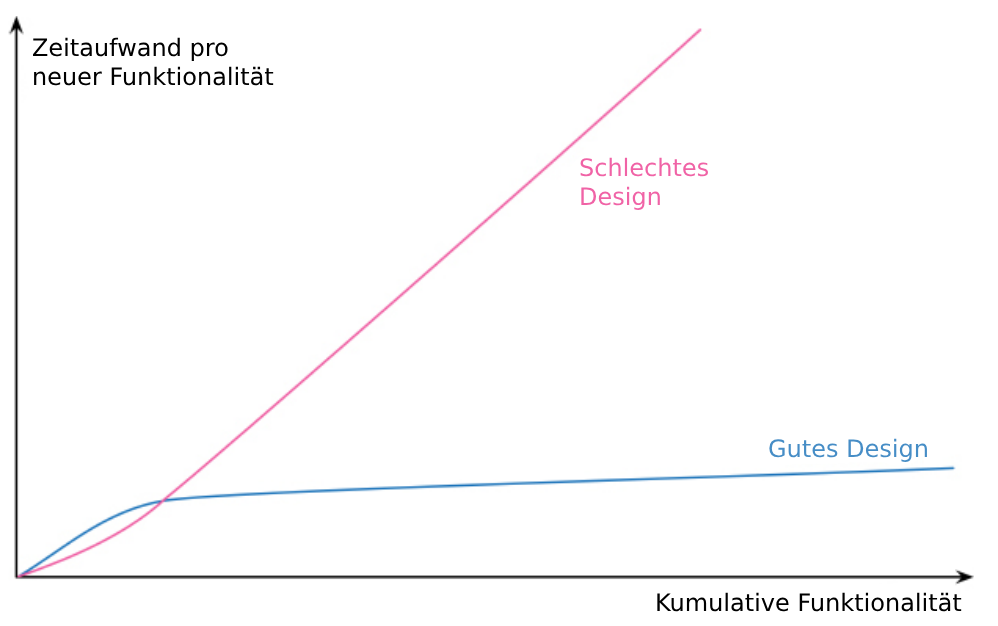
\includegraphics[width=\linewidth]{images/FowlerChart.png}
  \caption{Illustration zum Verhältnis von Funktionalität und Zeitaufwand nach \cite{fowler2019refactoring}}
  \label{fig:Refactoring_Graph}
  \Description{Illustration zum Verhältnis von Funktionalität und Zeitaufwand nach \cite{fowler2019refactoring}}
\end{figure}

Wie in Abb. \ref{fig:Refactoring_Graph} illustriert, können wir den Zeitaufwand für neue Features durch gutes Design verringern. Einflussreiche Faktoren sind hier nicht nur sauberer Code, sondern auch klare Modularität.\cite{fowler2019refactoring}


\subsection{Methodik}\label{sec:Refactoring_Methodik}

Bevor die Methodik betrachtet wird, sollte die Notwendigkeit von Tests erwähnt werden. Diese stellen die wichtigste Grundlage für das weitere Vorgehen dar. Wie bereits in \ref{sec:Refactoring_Einführung} beschrieben, ist das Ziel von Refactoring nur den Code, nicht aber das Verhalten des Codes zu bearbeiten. Ob diese Anforderung erfüllt wird, lässt sich nur mit einer genügenden Test-Abdeckung absichern. Diese sollte weiterhin via Continuous-Integration in den alltäglichen Arbeitsprozess integriert werden, um sicherzustellen, dass an keiner Stelle neue Fehler auftreten. \cite{fowler2019refactoring}

Um das Vorgehen beim Refactoring zu verstehen, lohnt es sich, eine grobere Betrachtung und Kategorisierung vorzunehmen. Zu Beginn sollten wir zwischen 2 generell unterschiedlichen Arten des Refactorings differenzieren. \cite{inproceedingsHowWeRefactor} nutzt hierfür die Unterscheidung zwischen “Floss” (eng. Zahnseide) und “Root Canal” (eng. Wurzelkanal) Refactoring. Diese lautet wie folgt: Floss Refactoring ist Teil des stetigen Softwareentwicklungsprozesses und wird daher direkt in andere Entwicklungsprozesse mit integriert. Floss Refactoring stellt damit eine passive Aufgabe dar, die ohne explizite Erwähnung verfolgt wird. Root Canal Refactoring hingegen ist ein gesonderter Prozess, welcher als eigenständige Aufgabe erfolgt. Diese Art von Refactoring dient damit vor allem auch der Beseitigung schwerwiegenderer Missstände. Wie sich zeigen wird, ist es von großem Vorteil, die Menge an Floss Refactoring so gering wie möglich zu halten. \cite{articlePerspectives}
Unter Angesicht dieser Kategorisierung gibt es verschiedene methodische Empfehlungen. Generell gilt: Refactoring bietet sich oft am besten direkt vor einer Implementierung (oder einem Bugfix) an. Für Floss Refactoring bietet es sich ebenfalls an, opportunistisch zu handeln. Konkret bedeutet das, dass Entwickler immer dann, wenn sie Bedarf sehen, auch Refactoring anwenden. Diese Notwendigkeit kann sich z.B. durch ein Verlangen nach besserer Verständlichkeit oder der Reduktion von Komplexität äußern. Mit dieser Strategie ist es möglich, die Qualität des Codes als praktisch passiven Prozess zu verbessern.
Weiterhin empfiehlt \cite{fowler2019refactoring} geplante Refactorings (demnach also Root Canal Refactoring) so selten wie möglich anzusetzen. Tendenziell weisen diese eher auf größere Missstände hin. Auch gilt: Selbst wenn ein Root Canal Refactoring notwendig wird, ist es möglich, diesen Prozess in Form von kleineren Refactors umzusetzen. Diese können in gewisser Weise mehr wie Floss Refactoring betrachtet werden.
Zu guter Letzt gibt es auch Szenarien, in denen es sich nicht anbietet, ein Refactoring vorzunehmen. Namentlich betrifft dies vor allem Code, welcher so gravierende Probleme hat, dass ein Rewrite erforderlich ist. \cite{fowler2019refactoring}

\subsection{Umsetzung am Beispiel}

Um die theoretische Grundlage die in \ref{sec:Refactoring_Methodik} bereits beschrieben wurde zu untermalen sollen hier weitere Beispiele gegeben werden, wie ein Refactoring in der Praxis aussehen kann.
\cite{fowler2019refactoring} beschreibt eine breite Menge an möglichen Umsetzungen für konkrete Refactoring Maßnahmen.

\textbf{Encapsulate Variable}
Generell gilt dass Daten umständiger zu bearbeiten sind als Funktionen. Folgender Code kann sich vor allem bei wachsendem Programmumfang als problematisch darstellen:

\begin{lstlisting}[frame=single,breaklines=true]
class Student {
    public String StudentName;
}
\end{lstlisting}

Durch das ''Einkapseln'' dieser Variable ist es zukünftig einfacher an dieser Stelle Validations-Logik oder gar eine genaue Überwachung zu implementieren. Ebenfalls stellen wir so einen eindeutigeren Zugriffspunkt für diese Daten zur verfügung:

\begin{lstlisting}[frame=single,breaklines=true]
class Student {
    private String studentName;

    public String getName() {
        return this.studentName;
    }

    public void setName(String name) {
        this.studentName = name;
    }
}
\end{lstlisting}

Der Umfang dieses Refactorings enthält somit aber auch Änderungen an anderen Stellen im Code. Betroffen sind vor allen vorherige Zugriffe auf die öffentliche Variable, welche nun privat ist. \cite{fowler2019refactoring}

\textbf{Decompose Conditional}
In einem weiteren Beispiel aus \cite{fowler2019refactoring} wird auch die Komplexität angesprochen. Hier ist vor allem die Komplexität, die durch ''If-Conditions'' erzeugt wird von Interesse. So lässt sich leicht ein Szenario erdenken in welchem eine solche Kondition unnötig schwer zu verstehen ist:

\begin{lstlisting}[frame=single,breaklines=true]
if (date.isBefore(plan.summerBreakStart()) && date.isAfter(plan.summerBreakEnd)) {
    ticketFee = dayCount * plan.summerBreakFee + plan.regularCharge;
} else {
    ticketFee = dayCount * plan.semesterFee;
}
\end{lstlisting}

Dabei lässt sich diese Kondition auf Basis der Funktions-Extrahierung deutlich einfacher und lesbarer gestalten:

\begin{lstlisting}[frame=single,breaklines=true]
if (summerBreak()) {
    ticketFee = summerBreakCharge();
} else {
    ticketFee = regularCharge();
}
\end{lstlisting}

Hier extrahieren wir relevante Logik in verschiedenen Funktionen, welche durch ihre Benennung bereits den Zweck erahnen lassen. Die Logik dieser Kondition bleibt erhalten, ist allerdings deutlich einfacher zu lesen und kann somit auch schneller verstanden werden.

\subsection{Herausforderungen}\label{sec:Refactoring_Herausforderungen}

Die Anwendung von regelmäßigen Refactors ist nicht ohne Herausforderungen. In nicht unerheblichen Mengen an Softwareprojekten \cite{articlePerspectives} werden Refactorings aufgeschoben. Dies wiederum führt zu erheblichen Problemen:
\begin{itemize}
  \item Verringerte Produktivität
  \item Erhöhte Arbeitslast
  \item Höhere Fehleranfälligkeit
  \item Später anfallende hohe Arbeitslast durch notwendige Aufräumarbeiten
\end{itemize}
Gründe hierfür sind unter anderem, dass Produkte “schnell” entwickelt werden sollen, da der weitere Vertrieb an enge zeitliche Vorgaben gebunden ist. Dazu kommt, dass der Aufwand (auch “Kosten”) dieses Prozesses immer direkt geleistet werden muss, ohne dass dabei ein direkter ersichtlicher Vorteil besteht. Dieses Problem besteht primär für Entscheidungsträger, die nicht direkt mit dem Code in Berührung kommen. Da sich äußerliches Verhalten nicht ändert, ergibt sich leicht der Trugschluss, dass Refactoring keinen Wert zum Produkt hinzufügt. Aus dieser Betrachtungsweise ergibt sich nach \cite{articlePerspectives} vor allem bei der Priorisierung von Aufgaben ein Missstand. Entscheidungsträger priorisieren demnach vor allem neue Implementierungen und weisen Refactoring (aber auch Bugfixes) einen niedrigeren Stellenwert zu. Daraus ergibt sich ein Interessenkonflikt mit Entwicklern, die Refactoring tendenziell als wichtiger betrachten. Da Refactoring allerdings notwendig ist, um die Qualität des Codes bzw. des Produktes zu gewährleisten, gilt es diesem Problem entgegenzuwirken. Hierfür bietet es sich z.B. an, Entscheidungsträger enger in den agilen Planungsprozess zu integrieren. Dadurch erlaubt man einen besseren Wissensaustausch, welcher diesen Problemen entgegenwirkt.

Es gilt allerdings ebenfalls klarzustellen, dass Refactoring auch anderen Gefahren ausgesetzt ist. Neben unerfahrenen Entwicklern sind zu enge Zeitanforderungen ein weiteres Problem, welches zu ineffektiven bis hin zu fehlerhaften Refactorings führt. Weiterhin lohnt es sich auch hier wieder die absolute Notwendigkeit von Tests zu erwähnen, da der Mangel dieser ein erhebliches Risiko für die Anwendung von Refactoring bedeutet. \cite{articlePerspectives}


\subsection{Erfolgsfaktoren}\label{sec:Refactoring_Erfolgsfaktoren}

Um zu verstehen, wie man sich nicht nur den Herausforderungen aus \ref{sec:Refactoring_Herausforderungen} stellen kann, sondern auch generell Refactoring effektiv anzuwenden, ergeben sich aus \cite{6827119} verschiedene Erfolgsfaktoren. Diese beziehen sich generell auf alle Bereiche der agilen Softwareentwicklung. Hier wird auch besonders auf die Folgen für Softwarearchitektur geachtet. So werden die Erfolgsfaktoren primär darauf bezogen, ob kontinuierliches Refactoring zu einer zufriedenstellenden Architektur geführt hat. Daraus lassen sich verschiedene Unterpunkte ableiten, welche generell auf die agile Softwareentwicklung übertragen werden können:

\textbf{Projekt}
Die Geschwindigkeit, in welcher sich Anforderungen ändern, sollte nicht zu hoch sein. Ebenfalls sollten Implementierungen auch nicht schneller sein, als das Verständnis der Anforderungen reicht. Genauso ist es bei einer sehr geringen Rate an Veränderungen durchaus schädlich, kontinuierliches Refactoring zu betreiben.
Es gilt generell, dass kleinere Projekte mehr Erfolg haben. Bei größeren Projekten bietet es sich an, diese in kleinere Komponenten zu zerlegen.
Weiterhin ist ein entscheidender Faktor der bereits vorhandene architekturelle Wissensstand.
Ein letzter Punkt im Bezug auf Softwareprojekte ist deren Alter. Vor allem alte Projekte mit alten Architekturen erweisen sich in der Handhabung als deutlich komplexer.

\textbf{Team}
Wie bereits angesprochen, ist es für Entwicklungsteams von entscheidendem Vorteil, wenn mehr Erfahrung und Fähigkeiten vorhanden sind.
Ebenfalls von Relevanz ist die Einstellung der Teammitglieder im Bezug auf den Themenkomplex des Refactoring. Von Vorteil ist hier die Bereitschaft der Mitglieder sich anzupassen und zu lernen. Damit eng verbunden ist die Offenheit gegenüber der Wissensvermittlung und der damit einhergehenden Teamarbeit.
Zu große Entwicklungsteams sind hier von Nachteil.

\textbf{Praktiken}
Auch hier gilt erneut: eine automatische Testabdeckung ist von massivem Vorteil. Ein Mangel dieser Abdeckung führt vor allem in längeren Zeiträumen zu architektonischem Chaos. Damit einher geht die Anwendungen von Continuous Integration.
Zuletzt ist es hier auch von Vorteil, bereits gut etablierte Designprinzipien mit in die Entwicklung zu integrieren. Diese unterstützen den agilen Prozess und sorgen für Sicherheit.

\textbf{Organization}
Da Entscheidungsträger maßgeblichen Einfluss auf zeitliche Mittel haben, ist es von großem Nachteil, wenn diese zu eng arbeiten. Ein Mangel an Unterstützung, bzw. ein zu hoher Druck sorgt für Fahrlässigkeit der Entwickler.
Weiterhin ist es wichtig, eine kommunikative Unternehmenskultur zu etablieren, in der offen und ohne Schuldzuweisungen gearbeitet werden kann.

Neben den bereits genannten Faktoren ist es weiterhin von großem Vorteil, wenn es zu einem aktiven Wissensaustausch innerhalb der Entwicklungsteams kommt. Oftmals gibt es eine Dissonanz zwischen unerfahrenen und erfahrenen Entwicklern in Bezug auf die Notwendigkeit und Anwendung von Refactoring. Daher ist es von Vorteil, wenn erfahrene Entwickler ihren Wissensstand in Bezug auf das Refactoring aktiv an unerfahrene Entwickler weiterreichen. Dies kann z.B. in Code Reviews, aber auch in expliziten Guidelines erfolgen. \cite{6827119, fowler2019refactoring}

\section{Zusammenfassung und Diskussion}\label{sec:Zusammenfassung}

Technische Schulden betreffen jedes Softwareprojekt und gewinnen immer mehr an Bedeutung.
Von der ursprünglichen Auffassung Cunninghams bis zur modernen Betrachtung Fowlers hat
sich der Begriff TS stark gewandelt. Es ist jedoch nicht gewinnbringend, über Feinheiten
bei der Definition technischer Schulden zu diskutieren. Vielmehr muss das Konzept TS aktiv
wahrgenommen werden. Potentielle Gefahrenstellen müssen individuell im Projekt identifiziert
werden, sodass TS bewusst aufgenommen und auch behoben werden. Für einen erfolgreichen Umgang
mit TS bietet das Technische Schuldenmanagement sinnvolle Ansätze. Es umfasst die Identifikation,
Messung und Priorisierung technischer Schulden sowie die Prävention, Überwachung, Dokumentation,
Kommunikation und Rückzahlung. Automatisierte Tests, Code-Reviews und Coding-Guidelines können
bspw. bei der Prävention von Schulden helfen, wobei bestehende Schulden häufig mittels Refactoring
zurückgezahlt werden. In der Praxis wird eine erfolgreiche Umsetzung von TSM häufig durch eine
uneinheitliche Definition technischer Schuld, fehlende Tools sowie eine unzureichende
Kommunikation mit Entscheidungsträgern erschwert.

Der Lösungsansatz durch Refactoring stellt sich als integraler Teil in vielen erfolgreichen
agilen Prozessen dar. Er wirkt der Gefahr von technischen Schulden entgegen und sorgt gleichermaßen
für eine langfristig bessere Codequalität. Dabei ist die kontinuierliche Arbeit der Entwickler
mit einem klaren Fokus auf guten Code bzw. Architektur notwendig. Basis für all diese Arbeit
ist zwingender Weise eine automatische Testabdeckung. Ebenfalls müssen Unternehmensstrukturen
sowie Entscheidungsträger diese Notwendigkeit anerkennen und in ihre Prozesskette integrieren.
Wenn diese verschiedenen Aspekte auf Basis von angemessenen Design-Entscheidungen in den
Softwareentwicklungsprozess integriert werden, lässt sich die Chance drastisch erhöhen,
dass Projekte erfolgreich umgesetzt werden.

\section{Ausblick}\label{sec:Ausblick}

Die wissenschaftlichen Arbeiten zum Thema TS sind sehr jung. Die Anzahl der verfügbaren
Studien ist daher noch sehr gering. Erschwerend kommt hinzu, dass es keine einheitliche
Definition zu technischen Schulden gibt und je nach Quelle Feinheiten unterschiedlich
dargestellt werden. Außerdem ist es äußerst schwer, TS zu quantifizieren, wodurch das
Management dieser kompliziert wird. Dies könnte ein Ansatz für weitere Untersuchungen sein.
Für Refactoring ist es überaus schwierig, konkrete empirische Daten zu sammeln, welche den
direkten Einfluss belegen können. Dennoch gibt es verschiedene wissenschaftliche Arbeiten,
welche sich vor allem mit Erfahrungsberichten auseinandersetzen und daraus einen generellen
Kontext für positive und negative Faktoren ableiten. Bei diesen Ergebnissen fehlt es aber
an konkreten Vorgehensmodellen. Weiterhin ist das Thema der Planung von Refactoring im
Entwicklungsprozess zu großen Teilen unberührt und benötigt weitere Untersuchung.

%% The next two lines define the bibliography style to be used, and
%% the bibliography file.
\bibliographystyle{ACM-Reference-Format}
\bibliography{sample-base}

\end{document}
\endinput
%%
%% End of file `sample-acmtog.tex'.
